\documentclass{beamer}
\usepackage[utf8]{inputenc}
% \usepackage[T1]{fontenc}
% \usepackage[english]{babel}
\usepackage{wrapfig}
\usepackage{verbatim}
\usepackage{ mathrsfs }
\usepackage{dsfont}
\usepackage{amssymb}
\usepackage{amsmath}
\usepackage{amsthm}
\usepackage{graphicx}
\usepackage{lmodern}
\usepackage{float}
\usepackage{listings}
\usepackage{hyperref}
\usepackage{array}
\usepackage{multirow}
\usepackage{caption}
\usepackage{subcaption}
\usepackage{tikz}
\usetikzlibrary{positioning} 
\usetheme{Madrid}
\DeclareMathOperator*{\argmin}{argmin}
\DeclareMathOperator*{\argmax}{argmax}

\title{Inferring the underlying network of diffusion}

\begin{document}

\begin{frame}
\titlepage
\begin{figure}
    \centering
    
\includegraphics[scale = 0.5]{EPFL_Todai.jpg}
\end{figure}
\begin{tabular}{l}
     Supervisors :  \\
     Prof. Friedrich Eisenbrand\\
     Prof. Iwata Satoru\\
     Dr. Tasuku Soma
\end{tabular}
\hfill
\begin{tabular}{l}
     Student : \\
     Joachim Moussalli
\end{tabular}
\end{frame}

\begin{frame}{Table of Contents}
\tableofcontents
\end{frame}
\section{Introduction}
\begin{frame}{Motivation}
\begin{columns}
\column{0.5\textwidth}
(Fake) News
\column{0.5\textwidth}
\begin{figure}
    \centering
    
\includegraphics[scale = 0.1]{FakeNews.jpg}
\end{figure}
\end{columns}

\begin{columns}
\column{0.5\textwidth}
Marketing
\column{0.5\textwidth}
\begin{figure}
    \centering
    
\includegraphics[scale = 0.1]{Iphone.jpg}
\end{figure}
\end{columns}

\begin{columns}
\column{0.5\textwidth}
Diseases
\column{0.5\textwidth}
\begin{figure}
    \centering
    
\includegraphics[scale = 0.1]{diseases.jpg}
\end{figure}
\end{columns}
\end{frame}
\begin{frame}{Problem- Underlying network}
\begin{figure}
\begin{subfigure}{.4\textwidth}
    \centering
    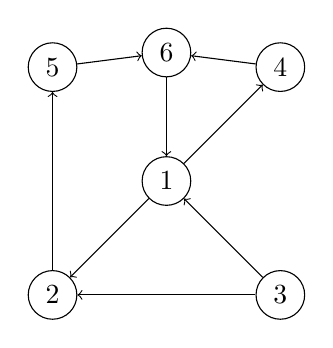
\begin{tikzpicture}[roundnode/.style = {circle, draw=black}]
     \node[roundnode] (1) {1};
     \node[roundnode] (2) [below left=of 1]{2};
     \node[roundnode] (3) [below right=of 1]{3};
     \node[roundnode] (5) [above left=of 1]{5};
     \node[roundnode] (4) [above right=of 1]{4};
     \node[roundnode] (6) [above=of 1]{6};
     
     \draw[->] (1)--(2);
     \draw[->] (1)--(4);
     \draw[->] (2)--(5);
     \draw[->] (3)--(1);
     \draw[->] (3)--(2);
     \draw[->] (4)--(6);
     \draw[->] (5)--(6);
     \draw[->] (6)--(1);
\end{tikzpicture}
\caption{Unkown underlying network,$G^* = (V,E^*)$}
\end{subfigure}
\begin{subfigure}{.4\textwidth}
    \centering
    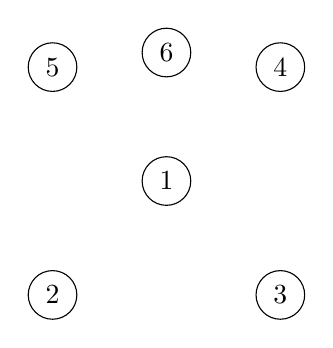
\begin{tikzpicture}[roundnode/.style = {circle, draw=black}]
     \node[roundnode] (1) {1};
     \node[roundnode] (2) [below left=of 1]{2};
     \node[roundnode] (3) [below right=of 1]{3};
     \node[roundnode] (5) [above left=of 1]{5};
     \node[roundnode] (4) [above right=of 1]{4};
     \node[roundnode] (6) [above=of 1]{6};
\end{tikzpicture}
\caption{Find the edges.}
\end{subfigure}
\end{figure}
\end{frame}
\begin{frame}{Problem- Cascades}
\begin{block}{Propagation Rules}
\begin{itemize}
    \item The infection is observed during a time window of length T,
    \item A vertex can only infect its neighbours,
    \item Once a vertex is infected it can not be infected again.
\end{itemize}
\end{block}
\begin{figure}
\begin{subfigure}{.4\textwidth}
    \centering
    \begin{tikzpicture}[roundnode/.style = {circle, draw=black}, infectednode/.style = {circle, draw=black, fill = green}]
     \node[roundnode] (1) {1};
     \only<4->\node[infectednode] (1) {1};
     \node[roundnode] (2) [below left=of 1]{2};
     \only<5-> \node[infectednode] (2) [below left=of 1]{2};
     \node[roundnode] (3) [below right=of 1]{3};
     \only<1>\node[roundnode] (5) [above left=of 1]{5};
     \only<2->\node[infectednode] (5) [above left=of 1]{5};
     \node[roundnode] (4) [above right=of 1]{4};
     \only<6->\node[infectednode] (4) [above right=of 1]{4};
     \node[roundnode] (6) [above=of 1]{6};
     \only<3->\node[infectednode] (6) [above=of 1]{6};
     \draw[->] (1)--(2);
     \only<5->\draw[thick,->] (1)--(2);
     \draw[->] (1)--(4);
     \only<6->\draw[thick,->](1)--(4);
     \draw[->] (2)--(5);
     \draw[->] (3)--(1);
     \draw[->] (3)--(2);
     \draw[->] (4)--(6);
     \draw[->] (5)--(6);
     \only<3->\draw[thick,->] (5)--(6);
     \draw[->] (6)--(1);
     \only<4->\draw[thick,->] (6)--(1);
\end{tikzpicture}
\end{subfigure}
\begin{subfigure}{.4\textwidth}
    \centering
    \begin{tikzpicture}[roundnode/.style = {circle, draw=black}, infectednode/.style = {circle, draw=black, fill = green}]
     \node[roundnode] (1) {1};
     \only<4->\node[infectednode] (1) {1};
     \node[roundnode] (2) [below left=of 1]{2};
     \only<5-> \node[infectednode] (2) [below left=of 1]{2};
     \node[roundnode] (3) [below right=of 1]{3};
     \only<1>\node[roundnode] (5) [above left=of 1]{5};
     \only<2->\node[infectednode] (5) [above left=of 1]{5};
     \node[roundnode] (4) [above right=of 1]{4};
     \only<6->\node[infectednode] (4) [above right=of 1]{4};
     \node[roundnode] (6) [above=of 1]{6};
     \only<3->\node[infectednode] (6) [above=of 1]{6};
     \only<3-> \draw[->] (5)--(6);
     \only<4-> \draw[->] (5)--(1);
     \only<4-> \draw[->] (6)--(1);
     \only<5-> \draw[->] (5)--(2);
     \only<5-> \draw[->] (6)--(2);
     \only<5-> \draw[->] (1)--(2);
     \only<6-> \draw[->] (5)--(4);
     \only<6-> \draw[->] (6)--(4);
     \only<6-> \draw[->] (1)--(4);
     \only<6-> \draw[->] (2)--(0,-1)--(4);
\end{tikzpicture}
\end{subfigure}
\end{figure}
\only<1>{$\textbf{t}^1$ = $(t_1,t_2,t_3,t_4,t_5,t_6)$}
\only<2> {$\textbf{t}^1$ = $(t_1,t_2,t_3,t_4,0,t_6)$}
\only<3> {$\textbf{t}^1$ = $(t_1,t_2,t_3,t_4,0,1)$}
\only<4> {$\textbf{t}^1$ = $(2,t_2,t_3,t_4,0,1)$}
\only<5> {$\textbf{t}^1$ = $(2,3,t_3,t_4,0,1)$}
\only<6> {$\textbf{t}^1$ = $(2,3,t_3,4,0,1)$}
\only<7> {$\textbf{t}^1$ = $(2,3,\infty,4,0,1)$ is called a \textit{cascade}.}
\end{frame}
\begin{frame}{Problem formulation- Infectious rates}
\begin{block}{Definition}
To each pair of vertices $(i,j)$ a weight, $\alpha_{i,j} \geq 0$, corresponding to the infectious rate is associated. Let us denote the set of infectious rate by $\mathscr{A} = \{\alpha_{i,j}|(i,j)\in V \times V, i\neq j\}.$
\end{block}
\begin{block}{Remark}
\begin{itemize}
    \item There is an edge between node $i$ and node $j$ $\iff \alpha_{i,j} > 0$.
    \item The infectious parameter might be dynamic with respect to time, i.e $\alpha_{i,j} \leadsto \alpha_{i,j}(t)$.
    \item If $X{\sim} Exp(\alpha)$ then $E[X]=\frac{1}{\alpha}$. It is the \textit{expected waiting time}.
\end{itemize}
\end{block}

\end{frame}
\begin{frame}{Problem formulation}
\begin{block}{Problem 1- Discrete optimization}
Given a collection of cascade $C$ propagating over a set of vertices $V$, find the underlying network $G^*$.
\end{block}
\begin{block}{Problem 2- Continuous optimization}
Given a collection of cascade $C$, find the correct infection parameters set $\mathscr{A}$.  
\end{block}
\begin{figure}
    \centering
    
\includegraphics[scale = 0.08]{Detective_Pikachu_-_Character_artwork_01.png}
\end{figure}
\end{frame}

\section{Related work}
\begin{frame}{Related work}
\begin{block}{Solutions of Problem 1}
\begin{itemize}
    \item \cite{NetInf} and \cite{MultiTrees} developed \textit{NetInf} and \textit{MultiTrees} algorithms.
    \item Submodular optimization with greedy algorithm.
    \item Requires apriori knowledge of the number of edges.
    \item Hard/Not efficient to extend to the dynamic setting.
\end{itemize}
\end{block}
\begin{block}{Solution of Problem 2}
\begin{itemize}
    \item \cite{NetRate} and \cite{InfoPath} developed \textit{NetRate} and \textit{InfoPaths} algorithms.
    \item Convex optimization solved with CVX and stochastic gradient descent (SGD).
    \item Easily extendable to the dynamic setting and no apriori knowledge needed.
    \item Computation time is higher than NetInf.
    \item No convergence complexity proofs.
\end{itemize}
\end{block}
\end{frame}

\begin{frame}{Probabilistic modeling (Exponential case)}
\begin{itemize}
    \item \textbf{Likelihood of transmission} $j\rightarrow i$ : %ATTENTION : Does not mean that j is the FIRST to infect i.
    \begin{equation}
    \mathscr{L}(\alpha_{j,i}|t_i-t_j) = f_{\alpha_{j,i}}(t_i-t_j) = \begin{cases}
    \alpha_{j,i} e^{-\alpha_{j,i}(t_i-t_j)}     &  \text{if} t_j < t_i\\
    0    & \text{otherwise}
    \end{cases}
\end{equation}
\item \textbf{Cumulative density function (CDF)} :
\begin{equation}
    F(t_i-t_j;\alpha_{j,i}) = \int_{0}^{t_i-t_j}f_{\alpha_{j,i}}(t)dt = 1-e^{-\alpha_{j,i}(t_i-t_j)}
\end{equation}
\item \textbf{Survival function} of node $i$ by time $t_i$ (w.r.t node $j$):
\begin{equation}
    S(t_i-t_j;\alpha_{j,i})=\mathds{P}(t_j + X \geq t_i) = 1-F(t_i-t_j;\alpha_{j,i}) = e^{-\alpha_{j,i}(t_i-t_j)}
\end{equation}
\item \textbf{Instantaneous infection rate} :
\begin{equation}
    H(t_i|t_j;\alpha_{j,i}) = \frac{f_{\alpha_{j,i}}(t_i-t_j)}{S(t_i-t_j;\alpha_{j,i})} = \alpha_{j,i}
\end{equation}
\end{itemize}
\end{frame}

\begin{frame}{Example}
\end{frame}

\begin{frame}{Likelihood of an edge in a cascade}
\begin{block}{likelihood of an edge (j,i)}
A node gets infected once the \alert{first} parent infects it. The likelihood of parent j being the first parent of i is given by :
\begin{equation}
    f_{\alpha_{j,i}}(t_i-t_j) \prod_{j\neq k,t_k<t_i}S(t_i-t_k;\alpha_{k,i})
\end{equation}
Then the likelihood of node i getting infected at time $t_i$ by one of the previously infected nodes $(t_1,\dots,t_N|t_k<t_i)$ is given by :
\begin{equation}
    \sum_{j:t_j<t_i}f_{\alpha_{j,i}}(t_i-t_j)\prod_{j\neq k,t_k<t_i}S(t_i-t_k;\alpha_{k,i})
\end{equation}
\end{block}
\end{frame}
\begin{frame}{Likelihood of a cascade}
\begin{block}{Infected nodes}
$\textbf{t}^{\leq T} = \{t_1,\dots,t_N|t_i\leq T\}$
    \begin{equation}
        \begin{split}
            \mathscr{L}(\mathbf{t}^{\leq T};\mathscr{A}) &= \prod_{i:t_i \leq T}\sum_{j:t_j<t_i}f_{\alpha_{j,i}}(t_i-t_j)\prod_{j\neq k,t_k<t_i}S(t_i-t_k;\alpha_{k,i})\\
            &= \prod_{i : t_i\leq T}\prod_{k:t_k<t_i}S(t_i-t_k;\alpha_{k,i}) \sum_{j:t_j<t_i}\frac{f_{\alpha_{j,i}}(t_i-t_j)}{S(t_i-t_j;\alpha_{j,i})}
        \end{split}
    \end{equation}
\end{block}
\begin{block}{Total likelihood}
\begin{equation}
    \mathscr{L}(\textbf{t};\mathscr{A}) = \mathscr{L}(\textbf{t}^{\leq T};\mathscr{A}) \prod_{i:t_i\leq T}\prod_{m:t_m>T}S(T-t_i;\alpha_{i,m})
\end{equation}
Considering a finite collection of cascade $C = \{\textbf{t}^1,\textbf{t}^2,\dots\}$, the likelihood of the infectious parameters is given by $\prod_{c \in C}\mathscr{L}(\textbf{t}^c;\mathscr{A})$
\end{block}
\end{frame}
\begin{frame}{Inference problem}
    \begin{block}{Problem}
    Find the transmission rates $\alpha_{i,j} \in \mathscr{A}$ for every pair of nodes such that the likelihood is maximized.
    \begin{equation}
    \begin{split}
        &\min_{\mathscr{A}} -\sum_{c\in C}\log \mathscr{L}(\textbf{t}^c;\mathscr{A})\\
        &\text{s.t  } \alpha_{i,j}\geq 0, i,j = 1,\dots,N, i\neq j
    \end{split}
    \end{equation}

    \end{block}
\end{frame}
\begin{frame}{Properties}
        $\mathscr{L}(C;\mathscr{A}) = \sum_{c \in C}\Psi_1(\textbf{t}^c;\mathscr{A})+\Psi_2(\textbf{t}^c;\mathscr{A})+\Psi_3(\textbf{t}^c;\mathscr{A})$
    \begin{equation}
        \begin{split}
        &\Psi_1(\textbf{t}^c;\mathscr{A}) = \sum_{i:t_i\leq T}\sum_{m : t_m>T} \log S(T-t_i;\alpha_{i,m}) = \sum_{i:t_i\leq T}\sum_{m : t_m>T} \alpha_{i,m}(T-t_i)\\
       &\Psi_2(\textbf{t}^c;\mathscr{A}) = \sum_{i:t_i\leq T}\sum_{j:t_j<t_i}\log S(t_i-t_j;\alpha_{j,i}) = \sum_{i:t_i\leq T}\sum_{j : t_j<t_i} \alpha_{j,i}(t_i-t_j)\\
        &\Psi_3(\textbf{t}^c;\mathscr{A}) = \sum_{i:t_i\leq T}\log(\sum_{j:t_j<t_i}H(t_i-t_j;\alpha_{j,i})) = \sum_{i:t_i\leq T}\log(\sum_{j:t_j<t_i}\alpha_{j,i}) 
        \end{split}
    \end{equation}
\end{frame}
\section{New algorithm}
\begin{frame}{Solving using ADMM}
    \begin{block}{ADMM for node i}
    Let $g_1(\textbf{t}^c;\Vec{\alpha_i}) = \sum_{j:t_j \leq T} \alpha_{j,i}(T-t_j) + \sum_{j : t_j<t_i} \alpha_{j,i}(t_i-t_j)$ and $g_2(\textbf{t}^c;z) = \log z $. The optimization problem reads now :
    \begin{equation}
        \begin{split}
            &\min_{\mathscr{A},z} -\sum_{c\in C}g_1(\textbf{t}^c;\Vec{\alpha_i}) +  g_2(\textbf{t}^c;z)\\
            &\text{s.t } z_c = \sum_{j:t_j<t_i}\alpha_{j,i} = M_c \alpha_i, \alpha_{k,i} \geq 0 \forall k\in V.
        \end{split}
    \end{equation}
    \end{block}
    \begin{block}{augmented lagrangian}
    \begin{equation}
        L_\beta(\alpha_i,z,\lambda) = g_1(\textbf{t}^c;\Vec{\alpha_i}) + g_2(\textbf{t}^c;z) + \lambda(M_c \alpha_i - z_c) + \beta/2||M_c\alpha_i -z_c||^2_2
    \end{equation}
    \end{block}
\end{frame}

\begin{frame}{ADMM iteration}
    \begin{block}{Iteration}
    \begin{equation}
        \begin{split}
            &\alpha_i^k = \min_{\alpha_i} -\sum_{c\in C} g_1(\textbf{t}^c;\Vec{\alpha_i}) + \lambda^{k-1}(M_c \alpha_i) + \beta/2 ||M_c\alpha_i - z_c^{k-1}||^2_2\\
            &z^k = \min_z -\sum_{c\in C} g_2(\textbf{t}^c;z) - \lambda^{k-1} z_c + \beta/2 ||M_c \alpha_i^k -z_c||_2^2\\
            &\lambda^k = \lambda^k + \beta(M\alpha_i^k - z^k)
        \end{split}
    \end{equation}
   \end{block}
    \begin{block}{Remark}
    Under the assumption that $g_1$ and $g_2$ are convex functions then, according to \cite{ADMM_Convergence}, ADMM converge in $O(1/t)$.
    \end{block}
\end{frame}
\section{Results}

\section{Conclusion}
\begin{frame}{Bibliographie}
    \bibliographystyle{plain}
    \bibliography{bibliographie}
\end{frame}
\end{document}
